\chapter{Grouping of object parts by motion for detection}
\label{chp4}
\section{Introduction}
% no \IEEEPARstart
% You must have at least 2 lines in the paragraph with the drop letter
% (should never be an issue)

\begin{comment}

Most state-of-the-art detection methods are based on the sliding-window schema~\cite{ac4,ac1} or the Hough transform~\cite{ac2,ac3,ac18}.
The sliding-window methods consider all sub-images by using classifiers to decide whether an object exists or not.
The Hough transform based methods, represented by the ISM~\cite{lb1}, start by detection of object parts, and object hypotheses are given by summing up all the votes voted by the object parts.
\end{comment}

\sout{In ITS areas, detection methods using cameras can be used for navigation, safe driving, surveillance, and sustaining results from other sensors. These methods can be used to detect pedestrians, bicycle riders, and automobiles, and here we focus on techniques from the area of computer vision for detection of such objects.}
{\color{red}In ITS areas, detection methods using cameras can be used for navigation, safe driving, surveillance, and sustaining results from other sensors. In traditional ITS applications, vehicles are main targets. Currently pedestrians are also considered as important subjects of ITS applications, and bicycles also become very popular for environmental and economical reasons. In Japan, the number of traffic accidents among bicycles and pedestrians is very large. Thus we tackle an issue of detecting freely moving bicycle riders and pedestrians from the data collected by a camera which keeps them under surveillance from the top. These situations can be observed in parks, university campuses, station squares, tourist spots, etc.  Here we focus on techniques from the area of computer vision for detection under surveillance scenarios.
\begin{comment}
Here we focus on techniques from the area of computer vision for detection of pedestrians and bicycle riders under surveillance scenarios.
\end{comment}
}




Most state-of-the-art visual
 detection methods fall into two main categories: sliding-window methods and Hough transform based methods. The methods~\cite{ac4,ac1} based on a sliding window schema perform detection in a typical machinery way. In these method, decisions of whether a target object exists or not are made for part of or all the sub-images in a test image. Beside the attractive performance and the extendibility of combining various kernels, these methods are favorable also because they consider each object as a whole during detection. However, they share limited aspects with visual perception in human beings, and the efficiency heavily relies on the size of the test images.

The other methods~\cite{lb1,ac2,ac3,ac18} detect objects based on the generalized Hough transform~\cite{ac17}. Object parts are detected, and the object parts provides confidence of locations being potential objects' centers. Locations of objects are decided according to the converged confidence. They are favorable for the robustness to partial deformation and easiness of training. To human beings, this kind of methods seems to be more natural. And in our work, we combine a mechanism of visual perception in human with the ISM~\cite{lb1} to demonstrate this natural property.





A typical Hough transform based method contains two steps: training and detection. During training, a codebook of object parts is built from a set of well annotated images. Each code in the codebook contains information about the appearance of the object part, the relative position to the object center, and the class label. Each object part's appearance is given in the form keypoint descriptors~\cite{lb1}, image patches~\cite{ac6,ac7}, or image regions~\cite{ac8}. Each code not only encode one object part's appearance, but also its offset to the \sout{the} object center and the class label. while during detection, on each test image, object parts are detected. Then every object part is matched against the codebook, and activates several nearest codes in appearance. The offset and class label encoded in each activated code will act as a vote. All the votes from the object parts are added up to form a Hough image. The peaks of the Hough image are considered as detection hypotheses with the height of each peak as the confidence for the corresponding hypothesis.

Two challenging issues for detection methods are how to separate near objects and how to separate similar different-class objects. The target objects, in the case of ITS applications, are pedestrians, bicycle riders, and automobiles. In the schema of sliding window, usually \sout{maximum}{\color{red}non-maximum} suppression is needed for post-processing, and a mechanism in ~\cite{ac4} works by excluding from the feature pool the features which belong to each successive found detection response. In Hough transform based methods, a similar mechanism is also employed in ~\cite{ac9}, however, this effort is after the forming of Hough image. During the forming of a Hough image, two kinds of votes make detection challenging: (1) votes casted by object parts from near objects make the peaks corresponding to different objects mixed up, and (2) votes casted by similar different-class object parts lead to tough decisions on the class label of the peaks. See Figure~\ref{fig:compa:c}. Before the forming of Hough images, problems also arise from the pollution of training images' background part to the codebook. During training a very clean codebook can be built with foreground marked, which needs manual efforts. Otherwise, large amount of training examples are needed for the effectiveness of the codebook, and this harms efficiency.


In videos, motion information is also available by simple tracking of object parts. Thus we propose a method for detection which utilizes both appearance and motion information. \sout{the}{\color{red}The} method is based on the common fate principle~\cite{ac13}. The principle is one of the visual perception principles as theorized by gestalt psychologists, and it states for human beings, tokens moving coherently are perceptually grouped. This provides an intuition to group the object parts by their motion patterns, and let them vote afterwards. In our work, the object parts are represented using keypoint descriptors, which are tracked to generate trajectories. The object parts are grouped by the pairwise similarities of their corresponding trajectories. Having the assumption that object parts in the same motion group  probably belong to the same object, for each object part, we assign higher weights for the votes of this object parts which are more {\lq\lq}agreeable{\rq\rq} within the motion group. This results in votes corresponding to true detection responses are more likely to be assigned higher weights. And on a Hough image formed by summing up these weighted votes, the peaks are easier to find as shown in Figure~\ref{fig:compa:d}.




\begin{figure}
\centering
\subfigure[]{
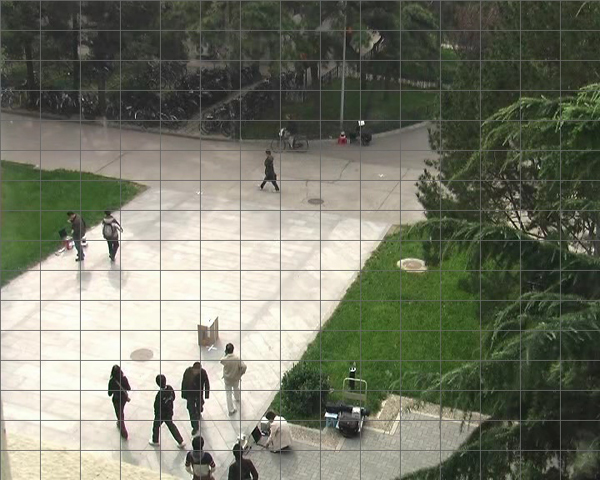
\includegraphics[width=0.48\textwidth,bb=0 0 600 480]{PEssR.jpg}
\label{fig:compa:a}}
\subfigure[]{
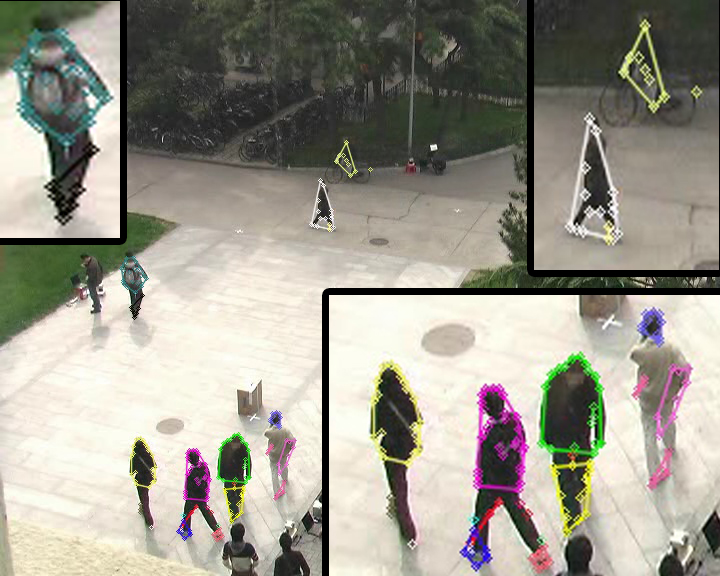
\includegraphics[width=0.48\textwidth,bb=0 0 720 576]{a56.jpg}
\label{fig:compa:b}}
\subfigure[]{
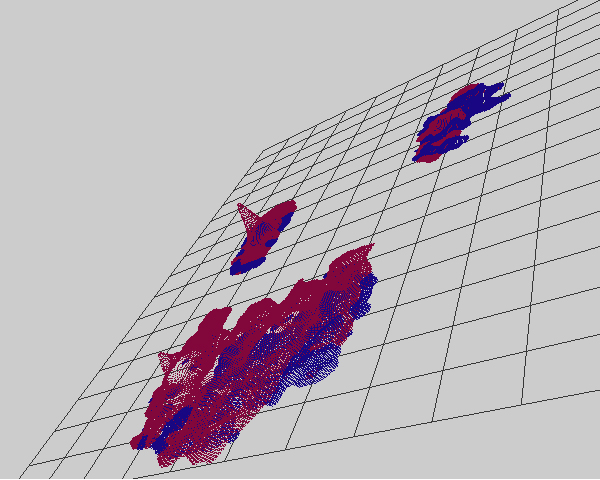
\includegraphics[width=0.48\textwidth,bb=0 0 600 480]{Untitled-6.jpg}
\label{fig:compa:c}}
\subfigure[]{
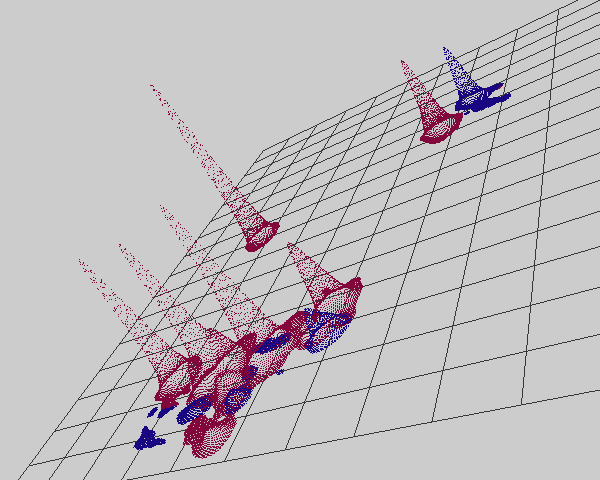
\includegraphics[width=0.48\textwidth,bb=0 0 600 480]{Untitled-4.jpg}
\label{fig:compa:d}
}
\caption{Merit of the proposed method. (a) Original image. (b) Motion \sout{group}{\color{red}grouping} results. {\color{red}Some parts are enlarged to show details.} (c) Original Hough image. (d) Hough image formed using our method. The grids in (c) and (d) correspond to the grids in(a).}
\label{fig:compa}
\end{figure}



By the combination of motion analysis results with the Hough transform framework through assigning different weights to each object part's votes, the proposed method has several appealing properties:
\begin{itemize}
\item {The method's ability to estimate object position and label of multiple objects from different classes. The existence of three types of objects makes the task challenging: near objects, similar different-class objects, and multi-pose same-class objects.}
\item {Its ability to use a codebook trained by images with cluttered backgrounds.}
\item {The framework to combine grouping results of object parts is very general, and has a good expandability.}
\end{itemize}

The remaining paper is organized as follows. Section 2 reviews related work. Section 3 gives formalism of the common fate Hough transform. Section 4 describes inference on the formed Hough images. Section 5 gives experimental results, and section 6 concludes.

\section{Related Work}

Our work is most related to object detection methods~\cite{ac9,ac22,lb1,ac5,ac10,ac21} based on the Hough transform framework. Recently, such methods make a lot of \sout{process}{\color{red}progress}. The ISM~\cite{lb1,ac5} is extended  by notifying correspondences between the object parts and the hypotheses~\cite{ac9} for the detection of multiple near objects. While in~\sout{\cite{ac10}}{\color{red}\cite{ac6,ac10,ac7}} the Hough transform is placed in a discriminative framework for object detection in a way that the codes are assigned different weights by the co-occurrence frequency of their appearance and offset to the object center.
Two Hough transform methods consider the grouping of object parts~\cite{ac26,ac25}. The method in~\cite{ac26} deals with scale change. Instead of estimating the scale by local features trained from different scaled examples, the votes are considered as voting lines. By considering the difference of the voted centers, local features are firstly grouped and then vote more consistently for the object center. In~\cite{ac25}, the grouping of object parts, the correspondence between object parts and object, and the decisions on detection hypotheses are optimized in the same energy function. For this method, the problem is that the grouping results don't have meaning or correspond to and real entities.

The work is also related to object detection methods by trajectories~\cite{my9,ac24}, methods weighting features~\cite{ij13}, methods dealing with codebook noise~\cite{ac19}, and methods which integrate temporal information~\cite{ac23}.

\section{Common Fate Hough Transform}
Probabilistic standpoints are very appealing, because of inference easiness. However, as pointed in~\cite{ac27}, placing the ISM in a probabilistic framework is not satisfactory. Especially, describing weights of the votes as priors does not make sense.
Hough transform can be simply considered as transformation from a set of  object parts, $\{\bf{e}\}$,  to a confidence space of object hypotheses, $C({\bf{x}},l)$. And $\bf{x}$ is the coordinate of the object center, while $l$ the label. Terms described as priors of the votes in the ISM are actually weights, and the likelihood terms are actually blurring functions to convert discrete votes into continuous space. Then this section describes how a Hough image for estimation of object centers and labels is formed from object parts observed on an image.


Let $\bf{e}$ denote an object part observed on the current image. The appearance of $\bf{e}$ is matched against the codebook, and $\bf{e}$ activates $N$ best matched codes from the trained codebook. Each code contains the appearance, its offset to the object center, and the class label. According to the $N$ matched codes, $\bf{e}$ casts $N$ votes. Each vote $V_{\bf{e}}$ is about the object center that generates $\bf{e}$. The position of the object center casted by  a vote, $V$, is denoted by ${\bf{x}}_V$, while the class label by $l_V$. Based on the $N$ votes of $\bf{e}$, the confidence that a position $\tilde{\bf{x}}$ is the center of an object with class label $\tilde{l}$ is given by,

\begin{equation}C({\tilde{\bf{x}}},\tilde{l};{\bf{e}}) = \sum\limits^N_{i=1} {B({\tilde{\bf{x}}},{\tilde{l}};{V_{\bf{e}}^i}) w({V_{\bf{e}}^i})}\:.
\label{eq1}
\end{equation}
Here $B({\tilde{\bf{x}}},{\tilde{l}};{V_{\bf{e}}^i})$ is the blurring function. And $w({V_{\bf{e}}^i})$ is the weight of ${V_{\bf{e}}^i}$.

The idea of the proposed method is that, the weight term, $w({V_{\bf{e}}^i})$, is defined by the motion grouping results of all the object parts.

The blurring function is defined as,

\begin{equation}
B(\tilde{\bf{x}},\tilde l;V)
= \left\{ \begin{array}{*{20}{c}}
   0   &\mbox{  if } {l_V} \ne \tilde{l} \mbox{ or } |\tilde{\bf{x}} - {\bf{x}}_V| > d   \\
   G(\tilde{\bf{x}};{{\bf{x}}_V},\sigma) &\mbox{otherwise}
\end{array} \right. \:.
\label{eq2}
\end{equation}
Here $G(\tilde{\bf{x}};{\bf{x}}_V,\sigma )$ is a Gaussian function that fixes the \sout{spacial}{\color{red}spatial} gap between $\tilde{\bf{x}}$ and ${\bf{x}_V}$.

Let $M$ be the total number of object parts on the image, then by summing up over all the object parts, the confidence of $\tilde{\bf{x}}$ being the center of a $\tilde{l}$-class object is given by,

\begin{equation}
\begin{aligned}
C({\tilde{\bf{x}}},\tilde{l}) &=\sum\limits^M_{j=1} C({\tilde{\bf{x}}},\tilde{l};{\bf{e}}_j)w({\bf{e}}_j) \\
&{
\begin{aligned}
=\sum\limits^M_{j=1} \sum\limits^N_{i=1} {B({\tilde{\bf{x}}},{\tilde{l}};{V_{{\bf{e}}_j}^i}) w({V_{{\bf{e}}_j}^i})w({\bf{e}}_j)} \:.
\end{aligned}
}
\end{aligned}
\label{eq3}
\end{equation}

Here, a uniform weight is assumed for each object part, and $w({\bf{e}}_j)=\frac 1 M$. Then by considering $C({\tilde{\bf{x}}},\tilde{l})$ as the evaluation score of the Hough space $({\tilde{\bf{x}}},\tilde{l})$, the task of estimating object centers and labels converts to finding and then validating the local maxima of the Hough image.

\subsection{Common Fate Weights}

To meet the challenges of separating near objects, separating similar different-class objects, and using a noisy codebook,  different weights are assigned to the votes of each object part by considering the motion grouping results of the object parts. In this sub-section, when given some grouping results, how the results are combined into a Hough transform framework is introduced.

Let $\gamma=\{\bf{g}\}$ denote the grouping results, where $\bf{g}$ is a group of object parts, and assume ${{\bf{e}}_m}\in \bf{g}$ and ${{\bf{e}}_n}\in \bf{g}$. Those votes of ${\bf{e}_m}$ which are more {\lq\lq}agreeable{\rq\rq} by the votes of the other objects in $\bf{g}$ are assigned larger weights.

Towards this end, the relationship between the votes of $\bf{e}_m$ and the votes of $\bf{e}_n$ needs to be given in advance. This relationship is named support. The support from ${V_{{{\bf{e}}_n}}}$ to ${V_{{{\bf{e}}_m}}}$ is defined by that based on ${V_{{{\bf{e}}_n}}}$, the confidence ${V_{{{\bf{e}}_m}}}$'s voted center is correct, as,


\[
S({V_{{{\bf{e}}_n}}} \to {V_{{{\bf{e}}_m}}})  =  B({\bf{x}}_{V_{{{\bf{e}}_m}}},l_{V_{{{\bf{e}}_m}}};{V_{{{\bf{e}}_n}}})\:,n \ne m\:.
\]
Here $B({\bf{x}}_{V_{{{\bf{e}}_m}}},l_{V_{{{\bf{e}}_m}}};{V_{{{\bf{e}}_n}}})$ is defined in (\ref{eq2}). This measures the coherence of the two votes from different object parts.

Then, the support from ${{\bf{e}}_n}$ to ${V_{{{\bf{e}}_m}}}$ is defined by that based on ${{\bf{e}}_n}$, the confidence that $V_{{{\bf{e}}_m}}$'s voted center is correct, as,

\[
\begin{aligned}
S({{{\bf{e}}_n} \to {V_{{{\bf{e}}_m}}}}) &= C({\bf{x}}_{V_{{{\bf{e}}_m}}},l_{V_{{{\bf{e}}_m}}};{{{\bf{e}}_n}})\\
& {
=\sum\limits^N_{i=1} {S({{V^i_{{{\bf{e}}_n}}} \to {V_{{{\bf{e}}_m}}}})w(V^i_{{\bf{e}}_n})}\:,n \ne m\:.
}
\end{aligned}
\]

And the support from ${\bf{g}}$ to $V_{{\bf{e}}_m}$ is defined by the confidence that $V_{{\bf{e}}_m}$'s voted center is correct based on the votes of all the other object parts but its belonging object part in $\bf{g}$, as,
\[
\begin{aligned}
S({\bf{g}} \to V_{{\bf{e}}_m})
&= \sum\limits_{{{\bf{e}}_i} \in {\bf{g}}- \{ {{\bf{e}}_m} \} }{C({\bf{x}}_{V_{{{\bf{e}}_i}}},l_{V_{{{\bf{e}}_m}}};{{{\bf{e}}_i}})w({{\bf{e}}_i})}\\
& =\frac 1 M  \sum\limits_{{{\bf{e}}_i} \in {\bf{g}}- \{ {{\bf{e}}_m} \}} {S({{{\bf{e}}_i} \to {V_{{{\bf{e}}_m}}}})} \:.
\end{aligned}
\]

\sout{By assuming all object parts in the same motion group are from the same object, which means motion grouping gives good results. The center position and the class label given by one vote shall be consistent with that given by the motion group.}{\color{red}By assuming all object parts in the same motion group are from the same object, which means motion grouping gives good results, the estimations for center position and class label given by every object part shall be consistent with that given by the motion group.}
Thus for a particular vote of ${\bf{e}}_m$, i.e., ${\tilde{V}}_{{\bf{e}}_m}$, a weight is assigned to it by considering its consistence with $\bf{g}$ and the consistence of ${\bf{e}}_m$'s other votes  with $\bf{g}$, as:
\begin{equation}
\begin{aligned}
{\color{blue}w(}&{\color{blue}{\tilde{V}}_{{\bf{e}}_m})}
= \frac
{S({\bf{g}} \to {{\tilde{V}}_{{\bf{e}}_m}}) + \frac{\Delta } N}
{\sum\limits^N_{i=1}{ S({\bf{g}} \to {V^i_{{{\bf{e}}_m}}})} + \Delta }\\
&
\begin{aligned}
= \frac
{ \sum\limits_{{{\bf{e}}_j} \in {\bf{g}}- \{ {{\bf{e}}_m} \}} {
\sum\limits^N_{k=1} {S({{V^k_{{{\bf{e}}_j}}} \to {{\tilde{V}}_{{{\bf{e}}_m}}}})\color{blue}{w(V^k_{{\bf{e}}_j})}}
}  + \frac{M\Delta } N}
{\sum\limits^N_{i=1}{
\sum\limits_{{{\bf{e}}_j} \in {\bf{g}}- \{ {{\bf{e}}_m} \}} {
\sum\limits^N_{k=1} {S({{V^k_{{{\bf{e}}_j}}} \to {V^i_{{{\bf{e}}_m}}}})\color{blue}{w(V^k_{{\bf{e}}_j})}}
}
} + M\Delta }\:.
\end{aligned}
\end{aligned}
\label{eq4}
\end{equation}
Here, $\Delta$ is a small constant for preventing zeros. Notice, $w({\tilde{V}}_{{\bf{e}}_m})$ is defined using $w(V^k_{{\bf{e}}_j})$, the weights of the votes of the other object parts in ${\bf{g}}$. In order to give $w({\tilde{V}}_{{\bf{e}}_m})$, uniform weights are firstly assigned to the votes of each object part in ${\bf{g}}$, i.e., $w(V^k_{{\bf{e}}_j})=\frac{1}{N}$. Then new weights are calculated based on the uniformly assigned weights. The weights of votes to form the Hough image are weights converged in iterations.

The grouping result $\gamma=\{\bf{g}\}$, can be replaced by grouping results based on other information, while our method utilizes motion to group the voting elements. The manner of extending the Hough transform is very general, and the extended Hough transform with motion grouping results is called the common fate Hough transform. The votes given by the best matched codes and the votes with higher defined weights are shown in Figure~\ref{fig:compa}.

\begin{figure}
\centering
\subfigure[]{
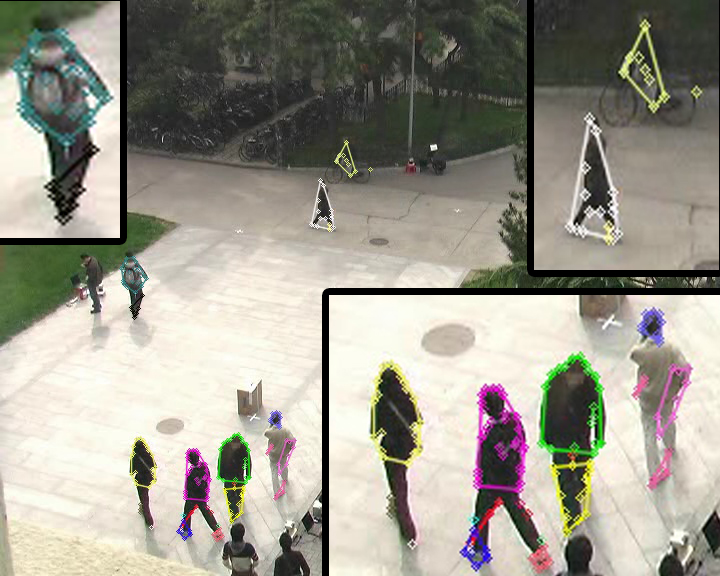
\includegraphics[width=0.47\textwidth,bb=0 0 720 576]{a56.jpg}
\label{fig:compa:a}}
\subfigure[]{
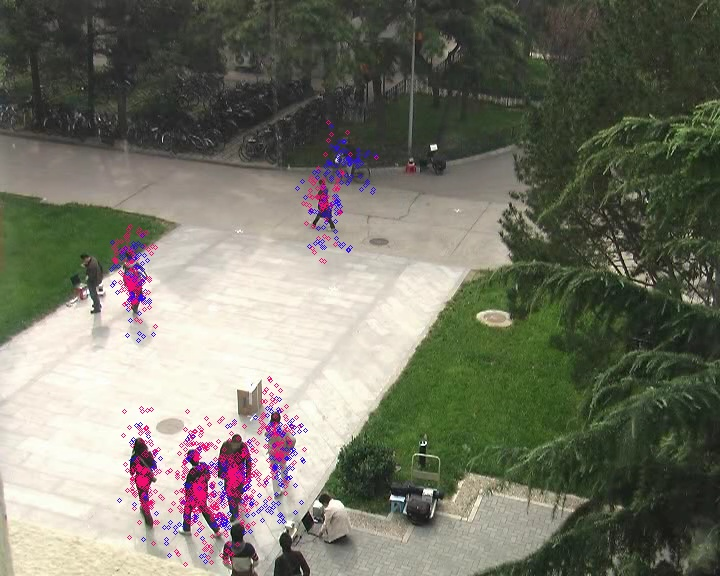
\includegraphics[width=0.47\textwidth,bb=0 0 720 576]{voteimg00056.jpg}
\label{fig:compa:b}}
\subfigure[]{
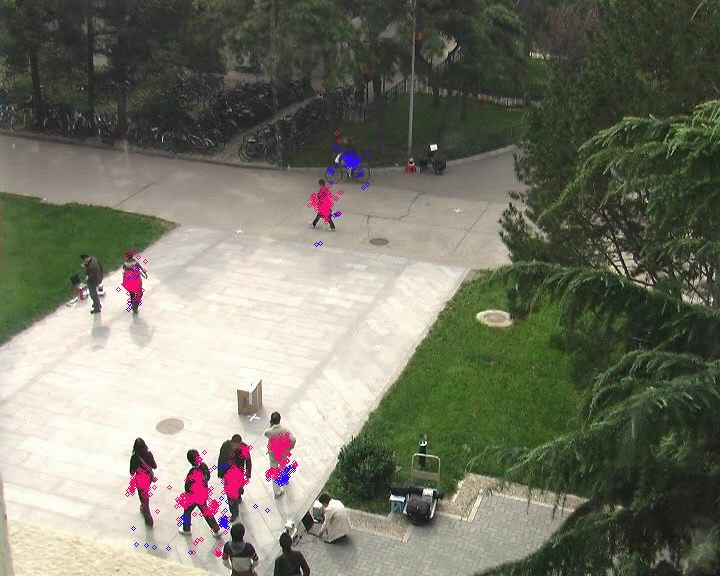
\includegraphics[width=0.47\textwidth,bb=0 0 720 576]{selectVimg00056_9.jpg}
\label{fig:compa:c}}
\subfigure[]{
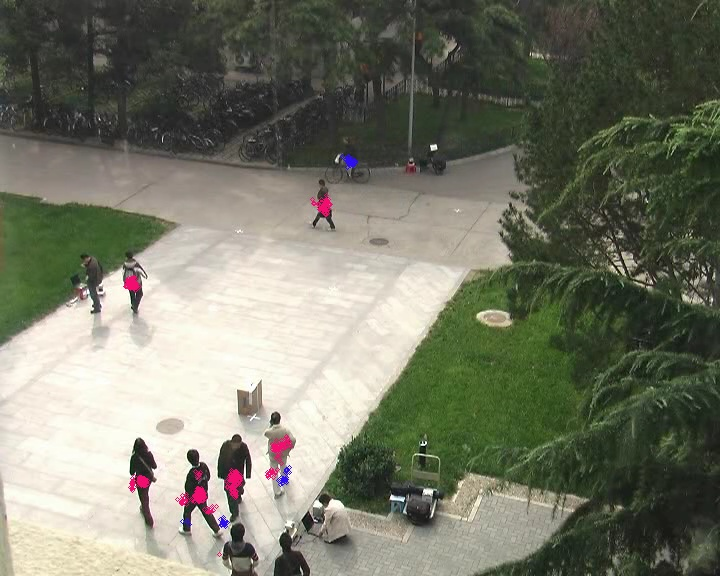
\includegraphics[width=0.47\textwidth,bb=0 0 720 576]{selectedvotesimg00056.jpg}
\label{fig:compa:c}}
\caption{Effect of the proposed weight. (a) Motion groups, different colors mark different motion groups. (b) Voted centers given by the 7 best matched codes. (c) Voted centers with the highest defined weights. (d) Voted centers with weights higher than a threshold.}
\label{fig:compa}
\end{figure}

\subsection{Motion Grouping}
In this subsection how to group the object parts by their motion patterns is introduced. Basically, the object parts are tracked, and clustered by their motion patterns. The object parts are tracked through frames before and after the current frame to generate trajectories. Then the object parts are grouped by their corresponding trajectories' pairwise motion similarity.

The object parts in this method are in the form of keypoint descriptors. The Harris Corner~\cite{harris} feature is chosen{\color{red}, for robustness,} to represent each object part, while for appearance, the region covariance~\cite{regionc} feature of the image patch around each keypoint is used. {\color{red}The image feature is chosen because of its flexibility to combine multiple channels of information, and also for its capability of handling scale changes in a certain range.}
For each object part, a trajectory is generated by tracking its corresponding Harris Corner by the KLT tracker~\cite{ij2}. To group the trajectories, two pairwise similarities are defined.

Let $T_{{\bf{e}}_m}$ and $T_{{\bf{e}}_n}$ denote two trajectories corresponding to ${{\bf{e}}_m}$ and ${{\bf{e}}_n}$. The first similarity between two trajectories is defined as,

\[
 {D_1}(T_{{\bf{e}}_m},T_{{\bf{e}}_n}) = \mathop {\max }\limits_{i=1...L} (|{\bf{x}}^i_{T_{{\bf{e}}_m}}-{\bf{x}}^i_{T_{{\bf{e}}_n}}|)\:.
\]

Here,  $i$ is the frame index, and $L$ is \sout{the length of the overlapping part of the two trajectories}{\color{red} the number of frames which are crossed by both trajectories}.

To define the second similarity, the $i$th directional vector of $T$ is firstly defined as, ${\bf{d}}^i_T={\bf{x}}^{i+3}_{T}-{\bf{x}}^i_{T}$. Let ${\bf{a}}_i={\bf{d}}^i_{T_{{\bf{e}}_m}}$, ${\bf{b}}_i={\bf{d}}^i_{T_{{\bf{e}}_n}}$, $a_i=\frac{{{{\bf{a}}_i}\cdot{{\bf{b}}_i}}}{{{{\bf{a}}_i}\cdot{{\bf{a}}_i}}}$, and $b_i=\frac{{{{\bf{a}}_i}\cdot{{\bf{b}}_i}}}{{{{\bf{b}}_i}\cdot{{\bf{b}}_i}}}$. Then the second similarity is defined as,
\[
{D_2}(T_{{\bf{e}}_m},T_{{\bf{e}}_n})= \mathop {\max }\limits_{i=1...L-3} (\max (|{{\bf{a}}_i} - a_i {{\bf{a}}_i}|,|{{\bf{b}}_i} - b_i{{\bf{b}}_i}|))\:.
\]

Before grouping the trajectories, the static points are excluded. \sout{Inspired by \cite{my9}, a minimal spanning tree of the trajectories is built upon $D_1$, and split by cutting edges larger than a threshold, $D^1_{th}$. For each element of the splitting results, a minimal spanning tree is built upon $D_2$ and split by cutting the edges larger than a threshold, $D^2_{th}$.}{\color{red} The defined $D_1$ is calculated for all pairs of trajectories, and a minimal spanning tree is then built using the calculated distances. The built mst is split by cutting edges larger than a threshold, $D^1_{th}$, and this gives a grouping result of the trajectories. For each element in the clustering result, $D_2$  is used in the same procedure to generate even smaller clusters.} This hierarchical procedure ensures that trajectories in the same group have both small $D_1$ and $D_2$. Each trajectory corresponds to an object part, and the grouping results of the trajectories correspond to grouping results of the object parts.
\subsection{Codebook}
For training, Harris corners are extracted from the training images with the object center and the class label annotated. In this method, region covariance is chosen to represent the appearance, which is defined as,
\[{\bf{r}} = \frac{1}{{K - 1}}\sum\limits_{i = 1}^K {({{\bf{z}}_i} - {\bf{\mu }}){{({{\bf{z}}_i} - {\bf{\mu }})}^T}} \;.\]
Here, $K$ is the number of pixels in the region, and ${{\bf{z}}_i}$ is a $7$-dimensional vector regarding the $(x,y)$ coordinate of the pixel, while ${\bf{\mu }}$ is the mean of ${{\bf{z}}_i}$.   And ${{\bf{z}}}(x,y)$ contains the RGB color of the pixel and the intensity gradients of the pixel, as: $r(x,y)$, $g(x,y)$, $b(x,y)$, $|\frac {\partial I(x,y)} {\partial x}|$, $|\frac{\partial I(x,y)}{\partial y}|$, $|\frac{{\partial ^2}I(x,y)}{\partial {x^2}}|$, and $|\frac{{\partial ^2}I(x,y)}{\partial {y^2}}|$.

The appearance similarity between ${\bf{r}}_m$ and ${\bf{r}}_n$ is given by,
\[
\rho ({\bf{r}}_m,{\bf{r}}_n) = \sqrt {\sum\limits_{i = 1}^7 {{{\ln }^2}{\lambda _i}} }\;.
\]
Here, $\lambda _i$ is the generalized eigenvalue by solving the generalized eigenvalue problem, ${\lambda _i}{\bf{r}}_m{{\bf{u}}_i} = {\bf{r}}_n {{\bf{u}}_i},{{\bf{u}}_i} \ne {\bf{0}}$, with ${\bf{u}}_i$ the eigenvector.

A square image patch around each keypoint is used to
represent the appearance of an object part. Six region co-
variances are generated for each image patch by using the
pixels of the top-left, the top-right, the bottom-left, the
bottom-right, the central, and all of the image patch. Then
besides the offset and the class label, a code contains six
region covariances. \sout{When an object part is matched against
the codebook, the similarity between the image patch of the
object part and a code is defined by the smallest similarity
of the corresponding region covariance. In this way,
a codebook of object parts is built.}{\color{red} All codes from all training images constitute the codebook. When an object part is matched against
the codebook, the similarity between the image patch of the
object part and a code is defined by the smallest similarity
of the corresponding region covariance.}
\section{Detection}
After forming the Hough image, the detection hypotheses are validated. Let ${\bf{h}}=\{ H \}$ be the points in the Hough space which are evaluated by $C({\bf{x}}_{H},l_{H})$ and have $C({\bf{x}}_{H},l_{H})>0$.  Inspired by~\cite{ac9}, the hypotheses are validated by an optimizing procedure. Let $O$ be the number of the points in ${\bf{h}}$. \sout{let}{\color{red}Let} $u_i=1\mbox{ or } 0$ indicate $H_i$ being a true object center or not. The problem is:
\[
\arg \max\limits_{u_i} \prod\limits_{i = 1}^O { C^{u_i}({H_i})} \Longleftrightarrow\arg \max\limits_{u_i} \sum\limits_{i = 1}^O {{u_i}\ln (C({H_i})} )\:.
\]
Let $v_{ij}=1\mbox{ or } 0$ indicate \sout{${e}_j$}{\color{red}${\bf{e}}_j$} belongs to $H_i$ or not, then
\[
\begin{aligned}
C(H_i)&=\sum\limits^M_{j=1} C({\bf{x}}_{H_i},l_{H_i};{\bf{e}}_j)w({\bf{e}}_j)\\
&=\frac 1 M \sum\limits^M_{j=1} v_{ij} C({\bf{x}}_{H_i},l_{H_i};{\bf{e}}_j)\:,
\end{aligned}
\]
and by assuming one object part belongs to and only belongs to one hypothesis, the problem is,
\[
\begin{aligned}
&\arg \max\limits_{u_i,v_{ij}} \sum\limits_{i = 1}^O {{u_i}\ln (\sum\limits^M_{j=1} v_{ij} C({\bf{x}}_{H_i},l_{H_i};{\bf{e}}_j)} )\\
&
\begin{aligned}
    s.t.:\mbox{ }&u_i=0\mbox{ or }u_i=1,\forall\;i;\\
    &v_{ij}=0\mbox{ or }v_{ij}=1,\forall\;i,\forall\;j;\\
    &\sum\limits_{i = 1}^O {v_{ij}}=1,\forall\;j;\;\;  \\
    &\sum\limits_{j = 1}^M {v_{ij}}\leq u_i,\forall\;i\:.
\end{aligned}
\end{aligned}
\]


Following~\cite{ac9}, the optimal result for the problem is given by greedy maximization. As described in Algorithm~\ref{alg:gm}, the largest local maximum of all the local maxima is chosen to be the center of a true object and then the object parts belonging to the chosen object center are excluded from the object part set. A new Hough image where new objects are found is formed using the remaining object parts. And this procedure ends when the object part set is empty or the confidence of the chosen object is lower than a threshold.

\begin{algorithm}[h]

    \caption{Greedy Maximization}
    \label{alg:gm}
     Let $\varepsilon$ be the set of object parts, $C_{th}$ be the low confidence threshold to accept detection responses, and $\hat{\bf{h}}$ be the local maxima of $\bf{h}$

     {\color{gray}
         \begin{algorithmic}[1]




        \WHILE {$\varepsilon \ne \emptyset$}

            \STATE Form $\bf{h}$ with $\varepsilon$\\

            \STATE Generate $\hat{\bf{h}}$ and select $H_i \in {\hat{\bf{h}}}, u_i=0$\\$ \mbox{ and } \forall {H^{'}} \in {\hat{\bf{h}}, C({\bf{x}}_{H_i},l_{H_i}) >= C({\bf{x}}_{H^{'}},l_{H^{'}}) } $
            \IF {$C({\bf{x}}_{H_i},l_{H_i}) >=C_{th}$}

                \STATE $u_i\leftarrow1$

                \FOR{${\bf{e}}_j\in \varepsilon$}

                    \IF{$\forall {H^{'}} \in {\hat{\bf{h}}}, C({\bf{x}}_{H_i},l_{H_i}|{\bf{e}}_j) >= $ \\\ $C({\bf{x}}_{H^{'}},l_{H^{'}}|{\bf{e}}_j)$}

                    \STATE $v_{ij}\leftarrow1$

                    \STATE $\varepsilon\leftarrow \varepsilon -\{ {\bf{e}}_j \}$

                    \ENDIF

                \ENDFOR

            \ELSE

                \FOR {${\bf{e}}_j \in \varepsilon$}

                \STATE $v_{1j}\leftarrow1$

                \ENDFOR

                \STATE $\varepsilon\leftarrow \emptyset$

            \ENDIF

        \ENDWHILE
    \RETURN $\{H_i,u_i=1\}$

    \end{algorithmic}
}
{\color{red}
    \begin{algorithmic}[1]




        \WHILE {$\varepsilon \ne \emptyset$}

            \STATE Form $\bf{h}$ with $\varepsilon$\\

            \STATE Generate $\hat{\bf{h}}$ and select $H_i \in {\hat{\bf{h}}} $ with the largest $   C({\bf{x}}_{H_i},l_{H_i})   $
            \IF {$C({\bf{x}}_{H_i},l_{H_i}) >=C_{th}$}



                \FOR{${\bf{e}}_j\in \varepsilon$}

                    \IF{$\forall {H^{'}} \in {\hat{\bf{h}}}, C({\bf{x}}_{H_i},l_{H_i}|{\bf{e}}_j) >= $ \\\ $C({\bf{x}}_{H^{'}},l_{H^{'}}|{\bf{e}}_j)$}



                    \STATE $\varepsilon\leftarrow \varepsilon -\{ {\bf{e}}_j \}$

                    \ENDIF

                \ENDFOR

            \ELSE



                \STATE $\varepsilon\leftarrow \emptyset$

            \ENDIF

        \ENDWHILE
    \RETURN $\{H_i\}$

    \end{algorithmic}
}
\end{algorithm}

\section{Experimental Results}
In experiments, improvement of the method is verified in terms of detection accuracy. The method is tested on the P-campus dataset with~\cite{ac9} as benchmark, and then tested on a dataset of \sout{sevral}{\color{red}several} animals.
\subsection{ Campus-scene Detection }
\begin{figure}
\centering
\subfigure[]{
\begin{minipage}[b]{0.47\textwidth}
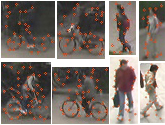
\includegraphics[width=1.0\textwidth,bb=0 0 165 125]{samples.jpg}
\end{minipage}
\label{fig:train:a}
}
\subfigure[]{
{
\begin{minipage}[b]{0.47\textwidth}
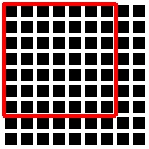
\includegraphics[width=0.3\textwidth,bb=0 0 149 149]{dst6.jpg}
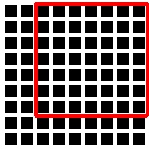
\includegraphics[width=0.3\textwidth,bb=0 0 149 149]{dst3.jpg}
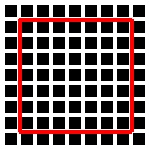
\includegraphics[width=0.3\textwidth,bb=0 0 149 149]{dst5.jpg}  \\
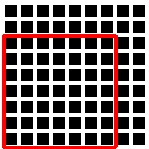
\includegraphics[width=0.3\textwidth,bb=0 0 149 149]{dst2.jpg}
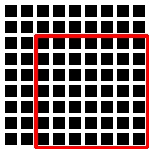
\includegraphics[width=0.3\textwidth,bb=0 0 149 149]{dst4.jpg}
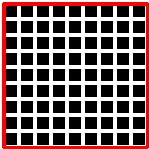
\includegraphics[width=0.3\textwidth,bb=0 0 149 149]{dst1.jpg}
\end{minipage}
}
\label{fig:train:b}
}
\caption{(a) Training images. Note some keypoints fall on the background. (b) The manner how a 9$\times$9 image patch is used to generate six region covariances, and red rectangles indicate the pixels used for each covariance.}
\label{fig:train}
\end{figure}

\textbf{Dataset} The P-campus dataset contains two primary classes of foreground objects: pedestrians and bicycle riders. The frame size is 720$\times$576. Among all the 401 continuous frames, 633 different-class ground truth bounding boxes are annotated on 79 frames. In this dataset, pedestrians and bicycle riders have in common the upper human body, and pedestrians appear in front, back, and side views.

\textbf{Implementation Settings} For training, 52 images of bicycle riders and 171 images of pedestrians are randomly selected. Harris corners are generated on the image, examples are given in Figure \ref{fig:train:a}. For appearance, six region covariances are generated for each keypoint using the 9$\times$9 image patch around it as shown in \ref{fig:train:b}. The appearance, the offset to the image (object) center, and the label of the training image are encoded into a code, and the code is inserted into a codebook. The final codebook contains 5502 codes.

\begin{figure}
\centering
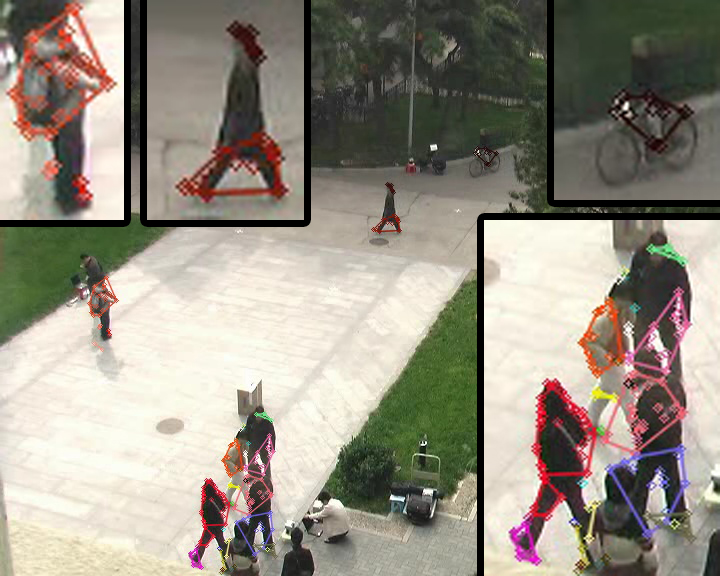
\includegraphics[width=0.47\textwidth,bb=0 0 720 576]{a16.jpg}
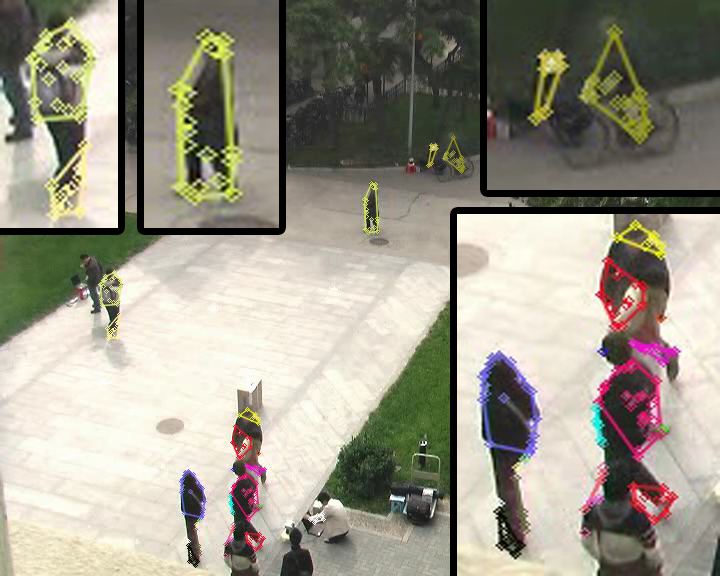
\includegraphics[width=0.47\textwidth,bb=0 0 720 576]{a26.jpg}
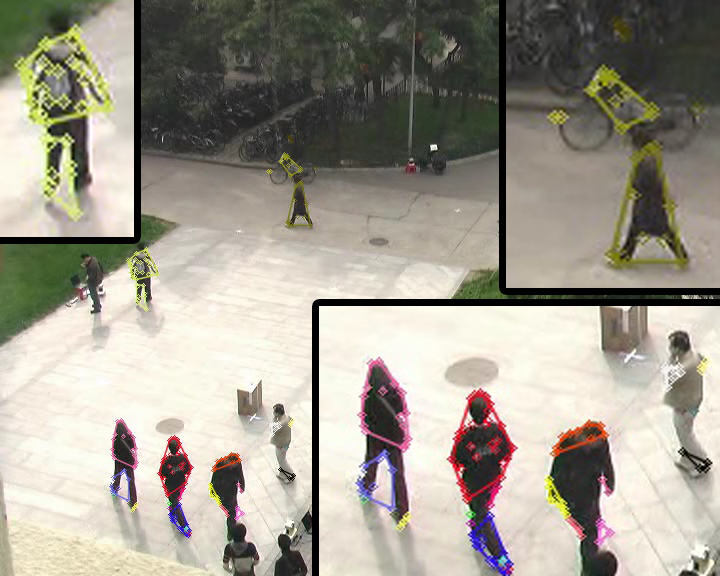
\includegraphics[width=0.47\textwidth,bb=0 0 720 576]{a71.jpg}
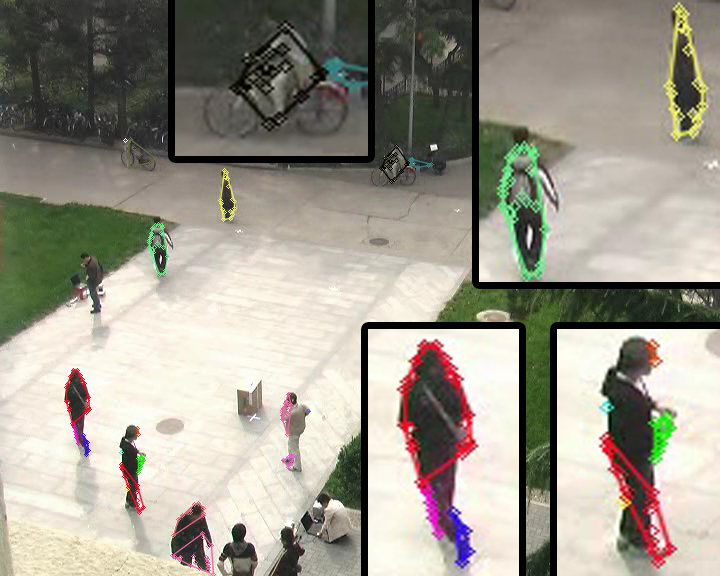
\includegraphics[width=0.47\textwidth,bb=0 0 720 576]{a116.jpg}
\caption{Motion grouping results.}
\label{fig:mgr}
\end{figure}

For motion grouping, each keypoint is tracked through 10 frames before and through 10 frames after the current frame. The similarity of two 21-point trajectories is defined using only \sout{the overlapping part}{\color{red} the frames crossed by both trajectories}. To set the two thresholds for motion grouping, $D_1$ and $D_2$ are  measured for keypoint pairs of different objects. $D^1_{th}$ is set that it is larger than only 10\% of the measured $D_1$s, and so is $D^2_{th}$. By doing so, keypoints belonging to different objects are not likely to be grouped together. So that in one motion group, the keypoints are very likely to belong to the same object, as shown in Figure \ref{fig:mgr}.

To form the Hough image, 35 best matched codes are chosen from the codebook for each object part. In (\ref{eq3}), $d$ and $\sigma$ need to be given. The precision-recall curves are based on $\sigma$, while $d$ is set to be 10. Here $\sigma$ is the most important parameter.

\textbf{Comparisons} For comparison, detection is done on the Hough images formed with and without motion grouping results. The same codebook and the same parameter settings are used for forming and searching over both Hough images. The votes of each object part are assigned uniform weights in the benchmark method, while weights defined in (\ref{eq4}) are assigned in the proposed method.
\begin{figure}
\centering
\subfigure[]{
\begin{minipage}[b]{0.47\textwidth}
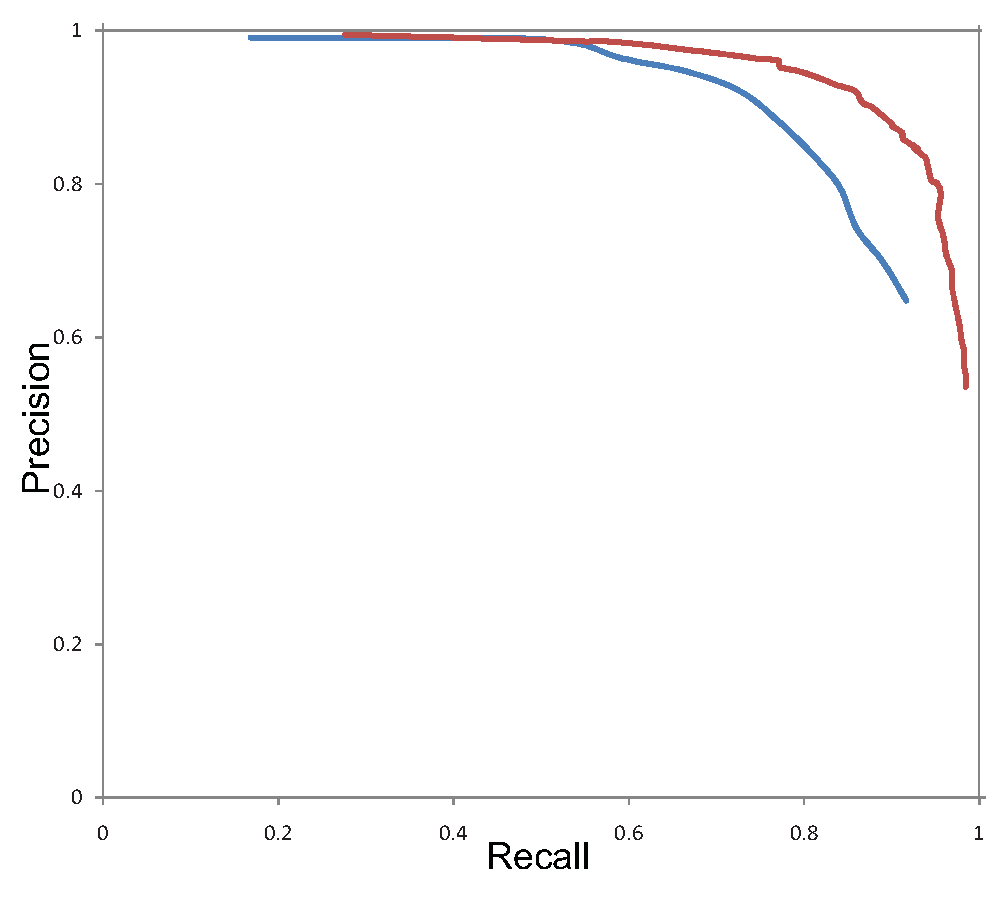
\includegraphics[width=1\textwidth,bb=0 0 480 425]{prf.eps}
\end{minipage}
\label{fig:pr:a}}
\subfigure[]{
\begin{minipage}[b]{0.47\textwidth}
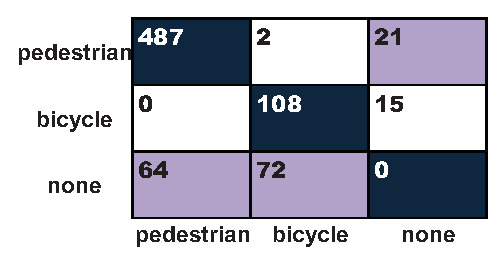
\includegraphics{cm2.eps}\\
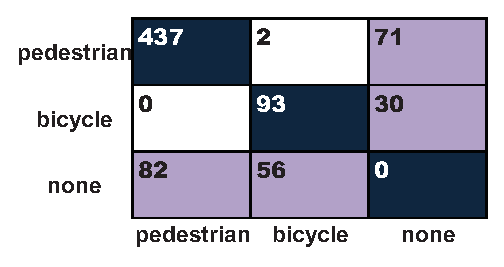
\includegraphics{cm1.eps}
\end{minipage}
\label{fig:pr:b}}
\caption{(a) Precision-recall curves (red: the proposed method, blue: the benchmark method). (b) Confusion matrices (upper: the proposed method, down: the benchmark method).}
\label{fig:pr}
\end{figure}



\begin{comment}
[width=1\textwidth,bb=0 0 480 425]
[width=\textwidth,bb=0 0 230 115]
[width=\textwidth,bb=0 0 230 115]
\end{comment}

The precision-recall curves are shown in Figure~\ref{fig:pr:a}. An object is considered as correctly detected only if the distance from the ground truth to it is less than 10 pixels. In Figure~\ref{fig:pr:a}, the correctly positioned but wrongly labeled objects are considered as true positives, aiming at verifying the positioning ability of the proposed method.

The confusion matrices are given in Figure~\ref{fig:pr:b}. For clarity of the comparisons, the proposed method is compared with the benchmark method when they have nearly equal number of false alarms. To evaluate the labeling ability, a class of {\lq\lq}none{\rq\rq} to represent missed detections and false alarms is manually added. For example, in Figure~\ref{fig:pr:b}, 487 pedestrian instances are correctly positioned and labeled by the proposed method, 2 are wrongly labeled to be bicycle riders, and 21 are miss-detected. More results are shown in Figure~\ref{fig:result}.

\begin{figure*}
\centering
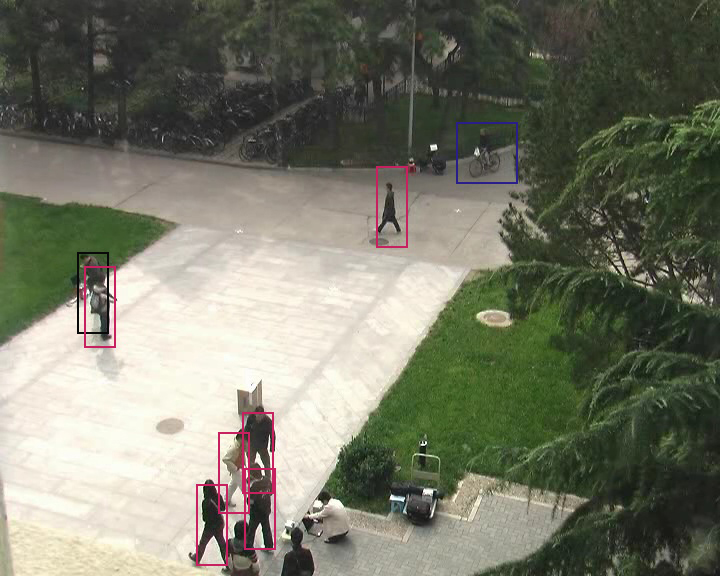
\includegraphics[width=0.47\textwidth,bb=0 0 720 576]{016.jpg}
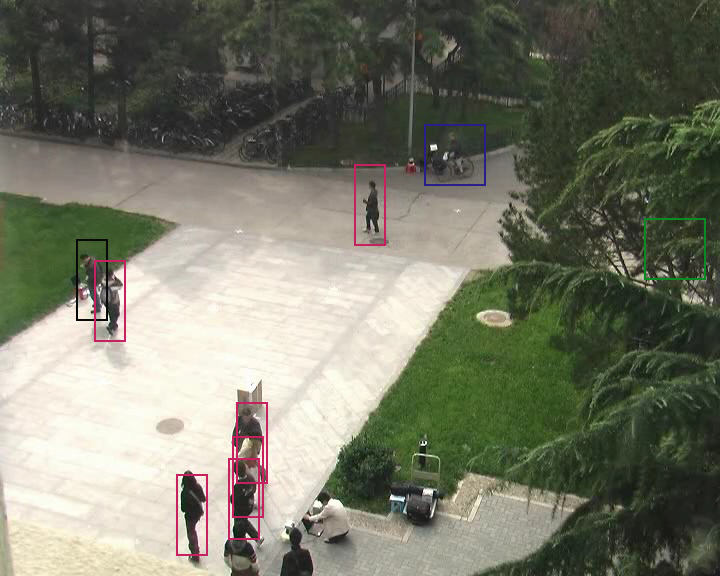
\includegraphics[width=0.47\textwidth,bb=0 0 720 576]{026.jpg}
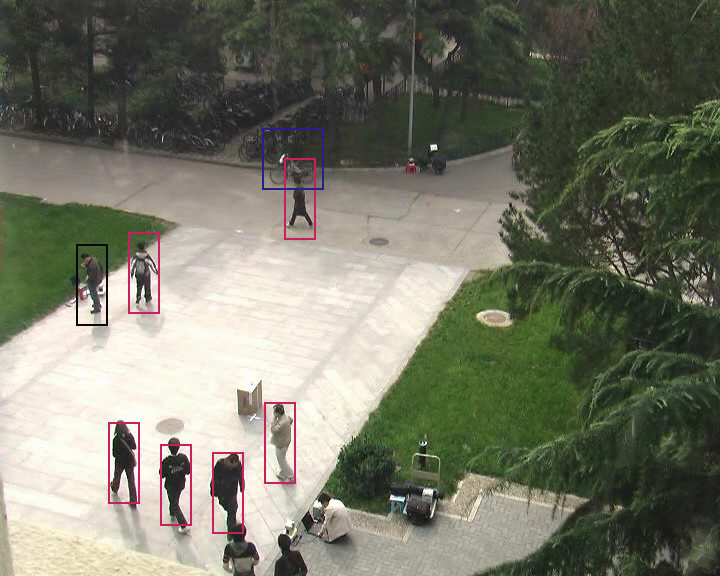
\includegraphics[width=0.47\textwidth,bb=0 0 720 576]{071.jpg}
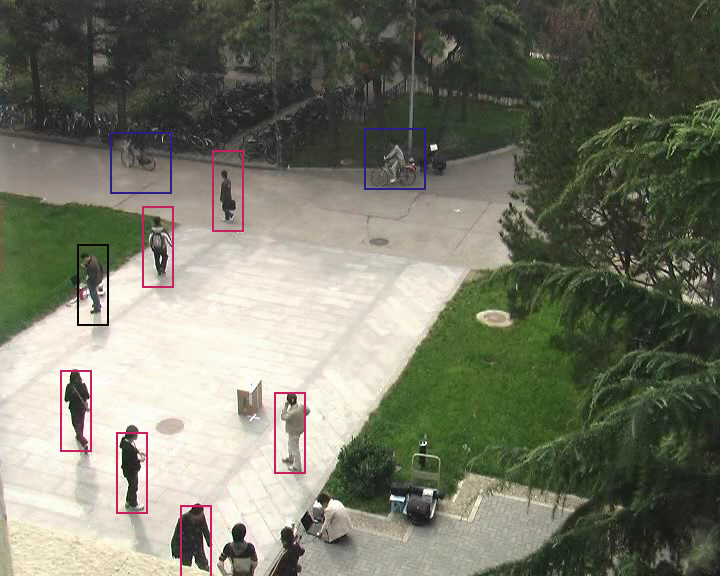
\includegraphics[width=0.47\textwidth,bb=0 0 720 576]{116.jpg}\\
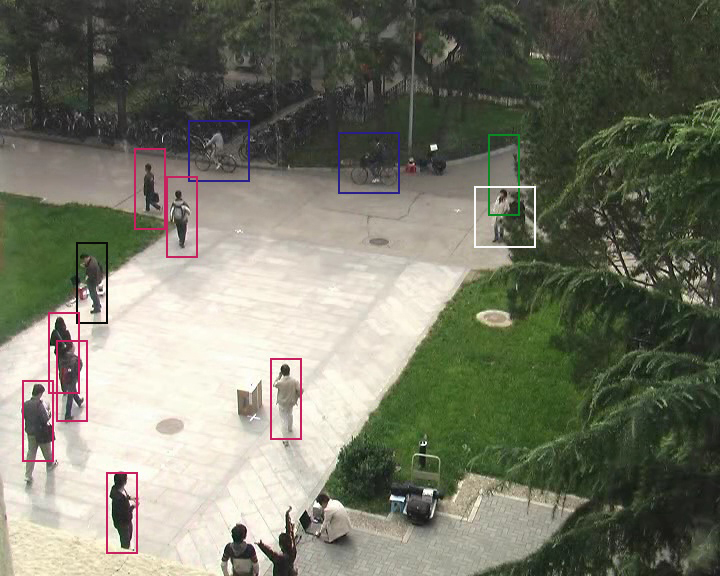
\includegraphics[width=0.47\textwidth,bb=0 0 720 576]{166.jpg}
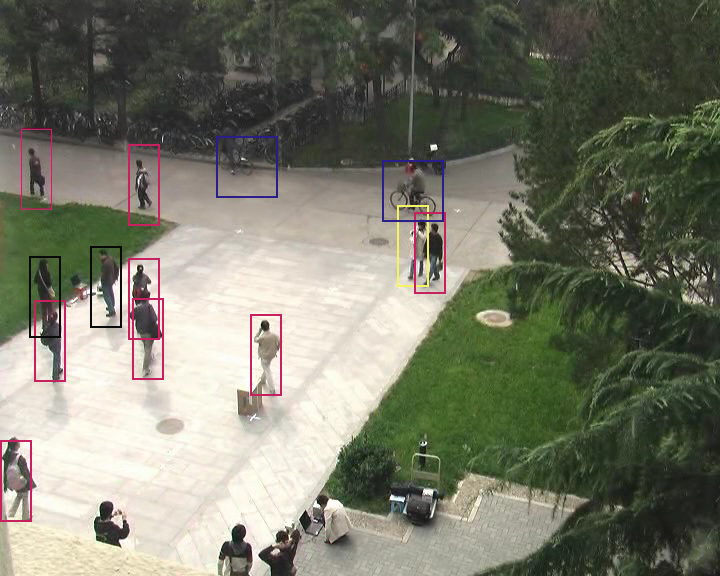
\includegraphics[width=0.47\textwidth,bb=0 0 720 576]{251.jpg}
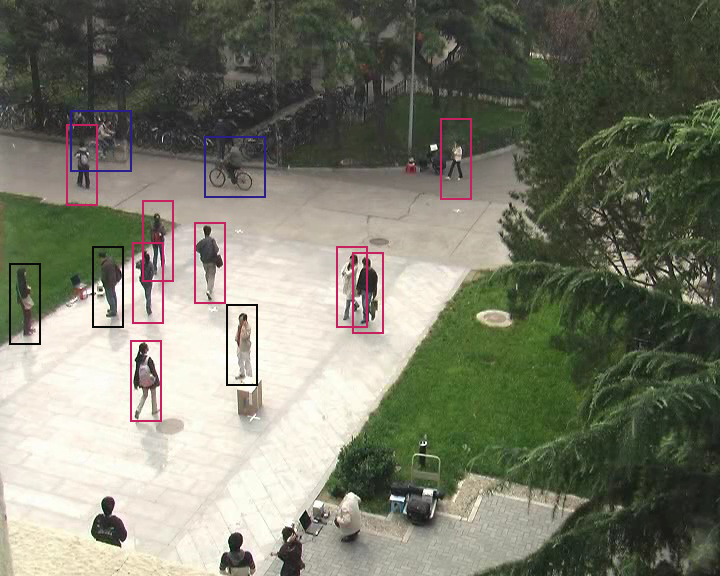
\includegraphics[width=0.47\textwidth,bb=0 0 720 576]{326.jpg}
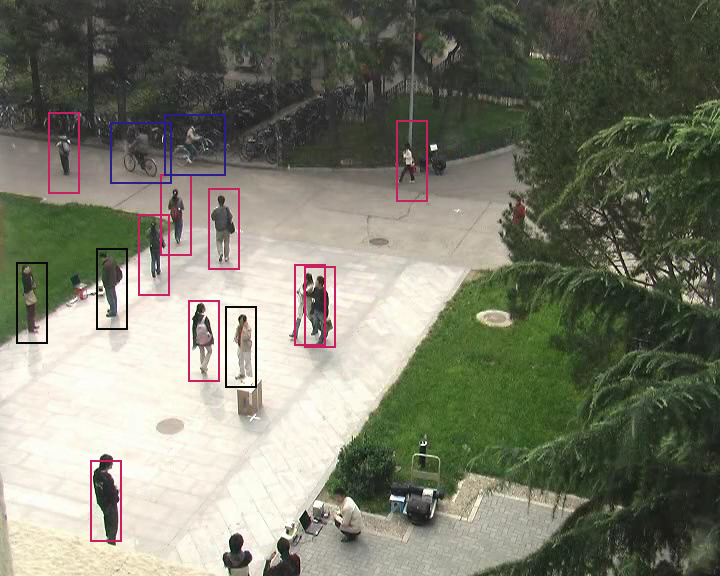
\includegraphics[width=0.47\textwidth,bb=0 0 720 576]{366.jpg}
\caption{Results. Red rectangles and blue rectangles mark correctly detected pedestrians and bicycle riders. Yellow rectangles mark missed detections. White rectangles mark correctly detected but not correctly labeled objects. Green rectangles mark false alarms. Black rectangles mark static objects, which are beyond the verification for the method.}
\label{fig:result}
\end{figure*}

\subsection{Wild-scene Detection}

\begin{figure}
\centering
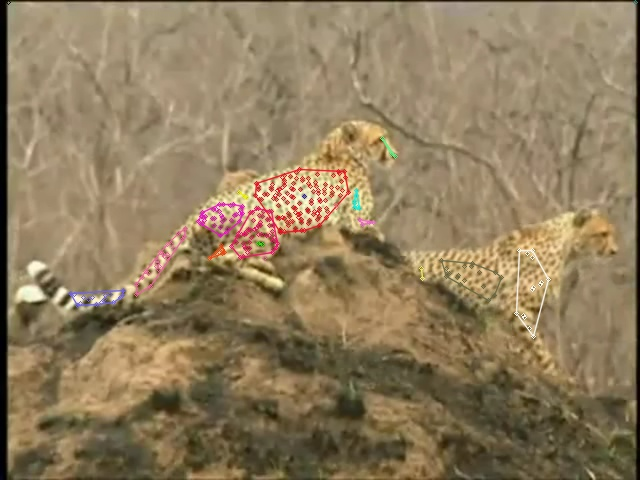
\includegraphics[width=0.47\textwidth,bb=0 0 640 480]{amotionimg00296.jpg}
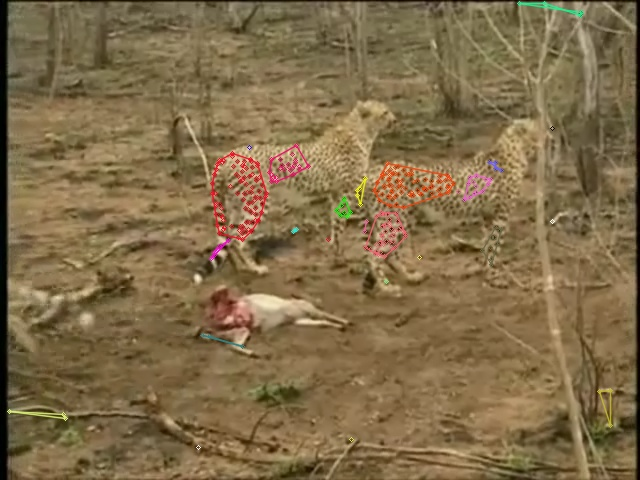
\includegraphics[width=0.47\textwidth,bb=0 0 640 480]{amotionimg01836.jpg}

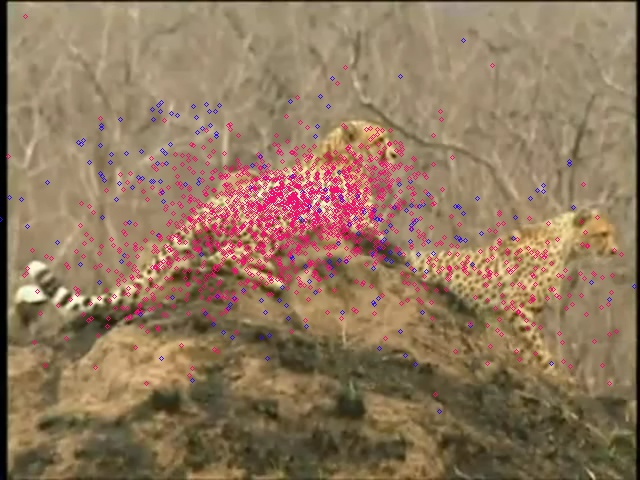
\includegraphics[width=0.47\textwidth,bb=0 0 640 480]{selectVimg00296_0.jpg}
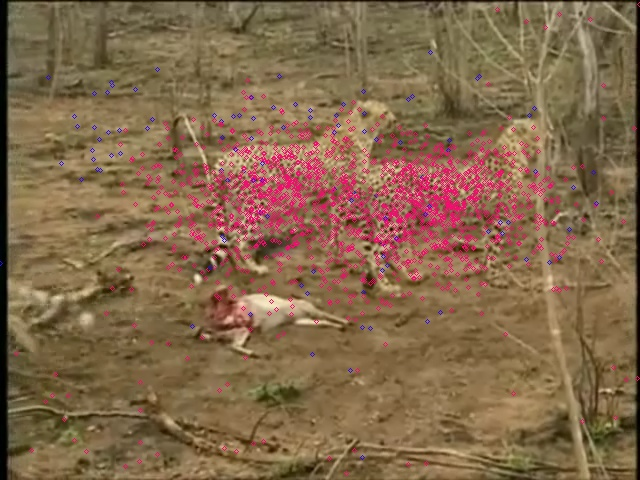
\includegraphics[width=0.47\textwidth,bb=0 0 640 480]{selectVimg01836_0.jpg}

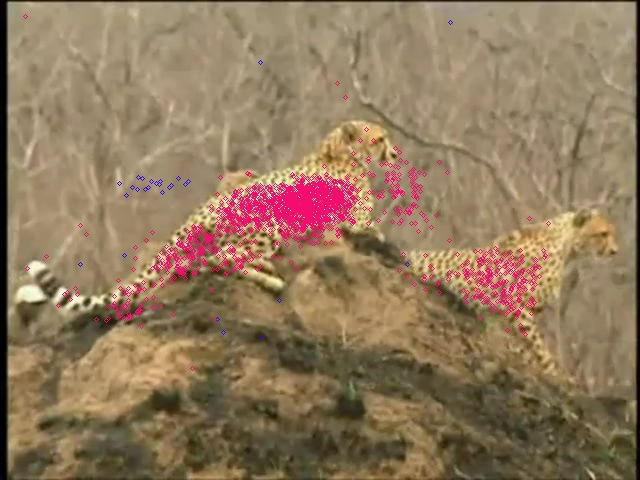
\includegraphics[width=0.47\textwidth,bb=0 0 640 480]{selectVimg00296_19.jpg}
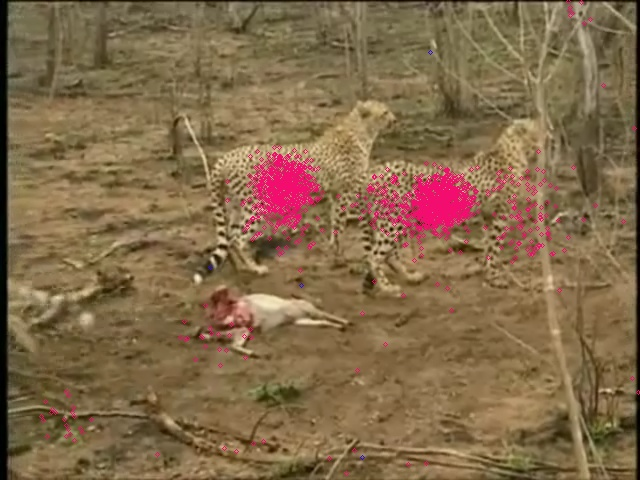
\includegraphics[width=0.47\textwidth,bb=0 0 640 480]{selectVimg01836_19.jpg}

\caption{Effect of the proposed weight assignment. Red circles are voted center for leopards, while blue ones are voted centers for tigers. On the top are the motion grouping results. In the middle are the voted centers according to the best matched codes. On the bottom are the voted centers voted by votes with highest weights.}
\label{fig:bcMP}
\end{figure}

\begin{figure}
\centering


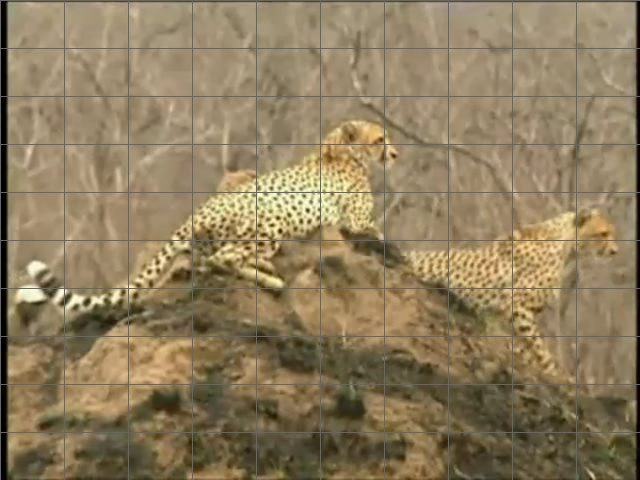
\includegraphics[width=0.47\textwidth,bb=0 0 640 480]{PER1.jpg}
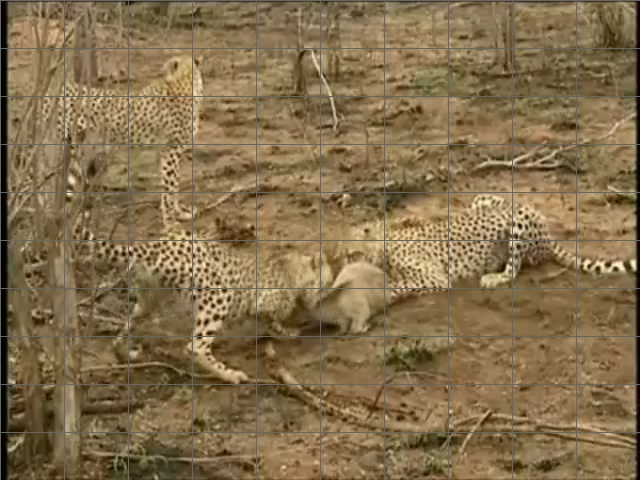
\includegraphics[width=0.47\textwidth,bb=0 0 640 480]{PER2.jpg}

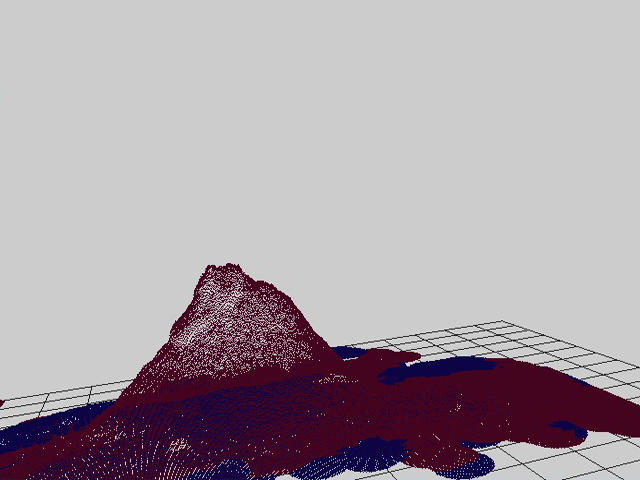
\includegraphics[width=0.47\textwidth,bb=0 0 640 480]{1.jpg}
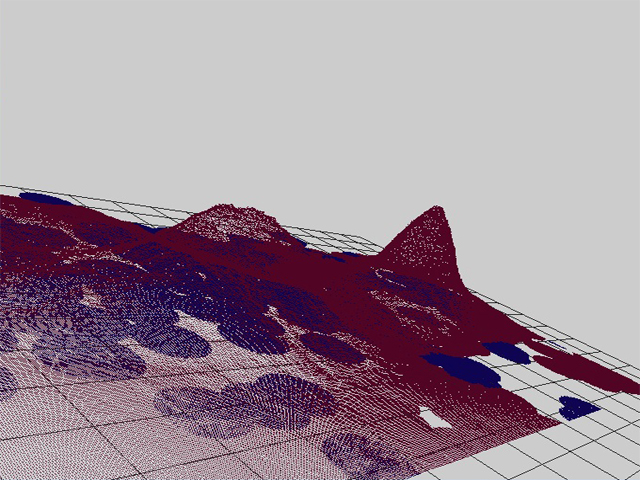
\includegraphics[width=0.47\textwidth,bb=0 0 640 480]{3.jpg}

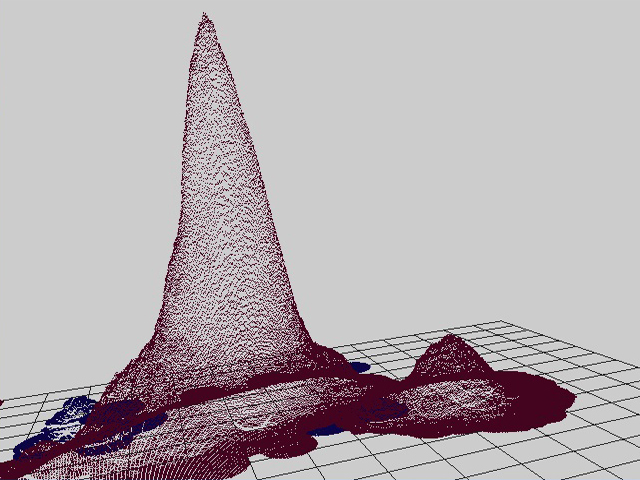
\includegraphics[width=0.47\textwidth,bb=0 0 640 480]{2.jpg}
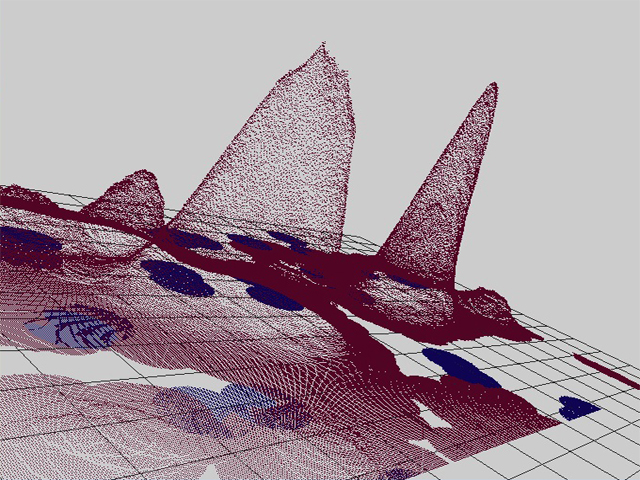
\includegraphics[width=0.47\textwidth,bb=0 0 640 480]{4.jpg}


\caption{Example Hough images. On the top are the original images. In the middle are the Hough images formed by votes with uniform priors. On the bottom are the Hough images formed by votes with the proposed weights. Red indicates leopards, and blue indicates tigers. Note for the two leopards, there is no peak corresponding to the right one on the benchmark Hough image. For the three leopards, there is also no peak corresponding to the leopard in behind on the benchmark Hough image.}
\label{fig:BcHi}
\end{figure}
\textbf{Dataset} \sout{To show the effectiveness of our method in general cases, we prepared a more difficult dataset.}{\color{red} In order to show that our method can be used for general purposes, we test our method on complicated scenes, especially, complicated background.  Even in these cases, our method works well, which shows robustness of our method.} A mini dataset is built upon leopards and tigers of the family Felidae. Especially, the image feature used by this method belongs to the type of texture, and texture from different \sout{postions}{\color{red}positions} of the leopards are almost the same. The dataset contains 6 video clips of 9 leopards and 4 tigers. The frame size is 640$\times$480. Both the animals are in the side view.

\textbf{Implementation settings} Most implementation settings are the same with the settings for campus object detection. For training, 5 leopards and 2 tigers are used. The size of the image patch around each keypoint is 27$\times$27.




\textbf{Comparisons} In Figure \ref{fig:bcMP}, the motion grouping results and how the voted centers are affected are given. Since parts from different positions of the leopard are very similar, the true center of a leopard is difficult to find from the voted centers of the object parts. In Figure \ref{fig:BcHi}, example Hough images are given to show the merit of the proposed prior by the ability to detect leopards. In Figure \ref{fig:bgdr}, the detection results are given. The proposed method successfully localizes and labels all the leopards and tigers, while the benchmark method miss-detects three leopards.

\begin{figure}
\centering
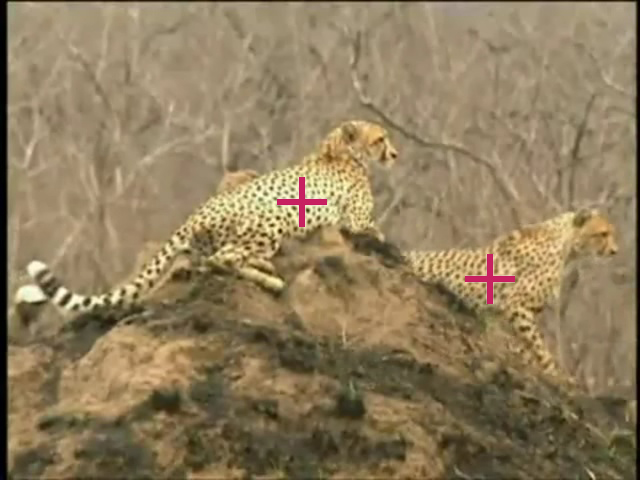
\includegraphics[width=0.47\textwidth,bb=0 0 640 480]{leo1.jpg}
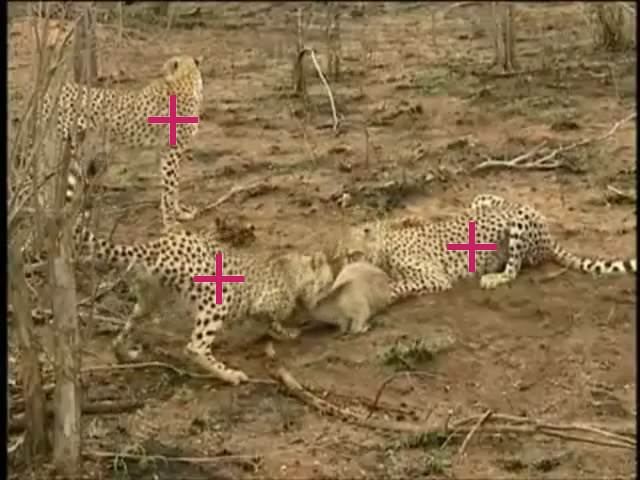
\includegraphics[width=0.47\textwidth,bb=0 0 640 480]{leo2.jpg}

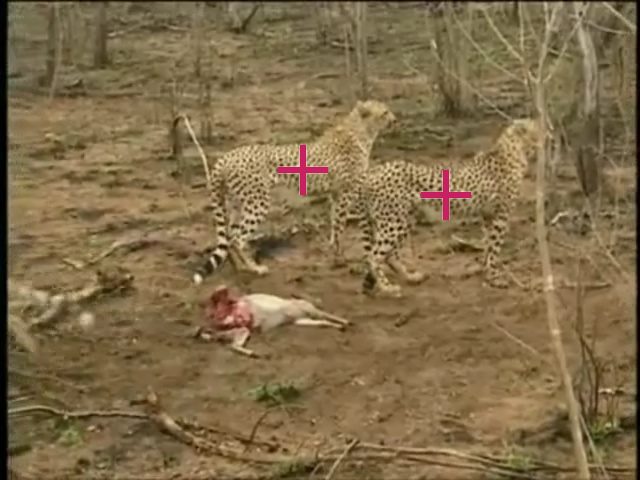
\includegraphics[width=0.47\textwidth,bb=0 0 640 480]{leo3.jpg}
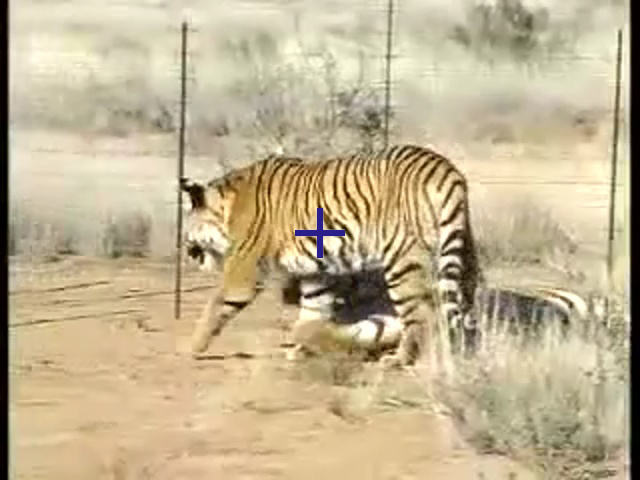
\includegraphics[width=0.47\textwidth,bb=0 0 640 480]{ti1.jpg}

\caption{Results. Red crosses mark the centers for leopards and blue crosses mark the centers for tigers.}
\label{fig:bgdr}
\end{figure}
\section{Conclusion}
The computational ability of human beings is limited, while the ability to detect is far beyond machines. Thus, it is very possible that this detection ability benefits from multiple perceptual mechanisms. By using one of these mechanisms, we propose a detection method. \sout{The}{\color{red}By embedding motion grouping results into the voting schema of hough transform, the} method is capable to distinguish near objects' positions, to distinguish similar objects' labels, and to maintain detection rate with a noisy codebook. The success of our method further demonstrate the advancement of perceptual mechanisms in human beings. And the success of this method will help with detection methods in ITS areas.
% conference papers do not normally have an appendix
